In order to determine which amino acids in a protein play the largest role in determining binding affinity it is convenient to compare the binding affinity of the native protein with that of a single residue mutant.
If the change in residue does not affect the folding of the protein, which with the exceptions of mutations to glycine, proline, or depending on the local structure possibly large amino acids, is unlikely. 
Alanine is the most frequently occurring amino acid, appearing in both solvent exposed and buried positions \cite{chothia1976nature,rose1985hydrophobicity}, and is unlikely to disrupt the protein fold in the same way glycine or proline might \cite{klapper1977independent}.
Additionally because it lacks a charge it does not interact electrostatically with the ligand.
These reasons makes it an attractive choice as a ``control'' amino acid for mutation scanning experiments.
Mutation scanning experiments, seek to identify residues which are have the largest contributions to binding affinity or ``hot spot'' residues.
By identifying single residue mutants which have a significantly decreased binding affinity when mutated to alanine \cite{cunningham1989high}.
\begin{figure}[h]
\centering
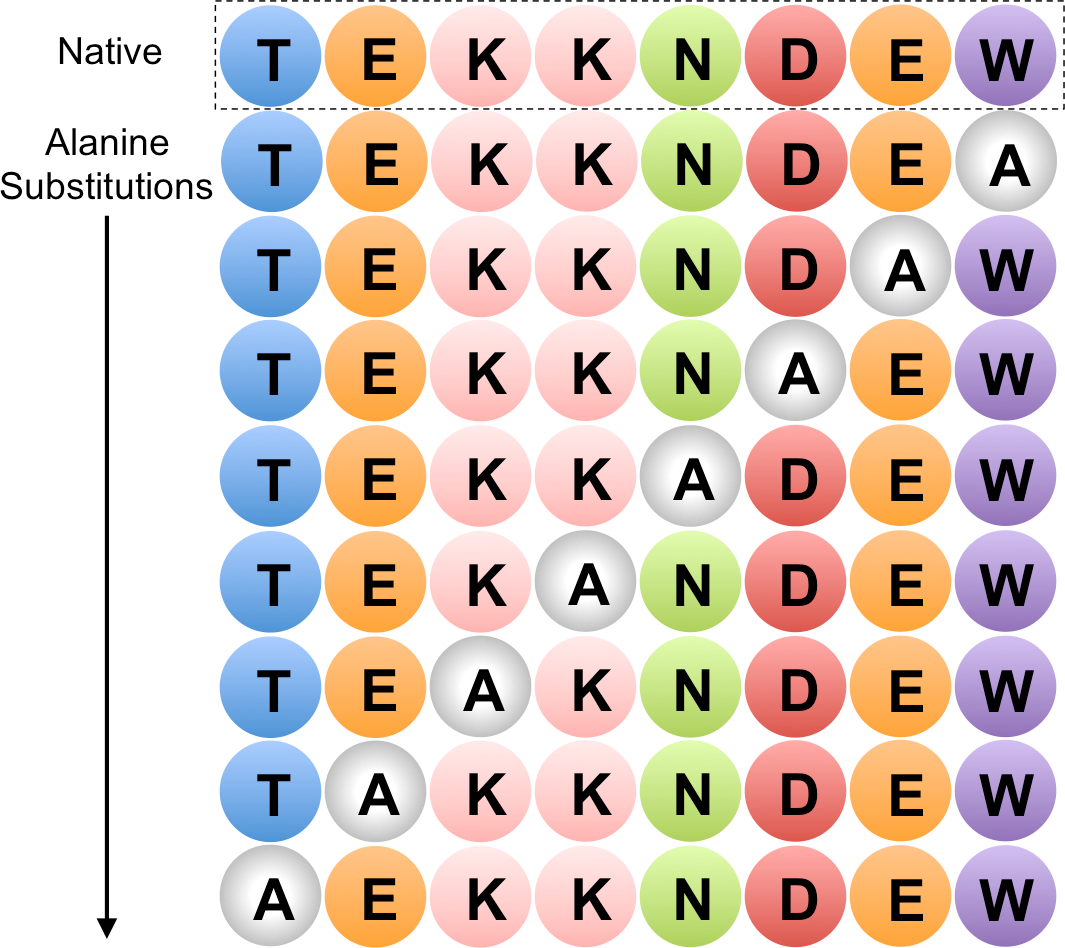
\includegraphics[width=0.5\textwidth]{figures/alanine_scan.png}
\caption{The sequences which would be evaluated during an alanine scan for Fc domain of a human IgG for streptococcal protein G.
The residues identified here were taken from the AESDB.
The native protein is represented in the top row \protect\cite{sauer1995crystal,thorn2001asedb}.
}
\label{fig:alanine_scan}
\end{figure}

The immune system maturation response, selects antibodies which have a reasonable affinity for an antigen, and creates a large number of variants of these antibodies. 
The effect of this is that the body produces antibodies with increasing affinity for an antigen some time after the initial exposure \cite{griffiths1984somatic}.
In vitro affinity maturation attempts to select molecules, frequently antibodies, with high affinity for some target molecule by creating a library of bacteria displaying variants of these antibodies on their cellular surface.
The means of doing this is bacteriophage display, which provides a method of pairing the protein represented on a bacterias surface with the genetic material contained by that bacteria \cite{smith1985filamentous}.
A bacteria is infected by a library of bacteriophages, containing a large number of variants of antibody of interest.
The phage will cause the bacteria to display their specific variant of the antibody on the bacteria surface, allowing sorting of the bacteria according to their affinity of the antigen, though affinity column purification or similar technique.
This step greatly enriches the fraction of antibody variants which bind the protein.
It is then possible to allow the bacteria to reproduce, sometimes causing more mutations to increase diversity of the antibody library and perform this affinity purification step again.
Sequential application of this affinity maturation makes it possible to identify a handful of antibody variants with high affinity from as many as $10^{6}$ different variants \cite{gram1992vitro,hawkins1992selection}.
However, the number of possible variants of the complementarity determining region (CDR) of an antibody many orders of magnitude larger than this.

Computational mutation scanning attempts to replicate the same sort of experiment {\it in silico}.
Making the same assumptions as above, namely that the backbone conformation is not altered by mutating a single residue to alanine, computational experiments attempt to identify hot spot residues by measuring the \ddg\ between the bound states of the native and mutated protein.

Mutated structures were generated by truncating side chain at C\subscript{$\gamma$} 
\cite{massova1999computational}

Varying cutoffs for {\it hot spot} residues are used, usually from 1.0 kcal/mol \cite{kortemme2002simple} to 4.0 kcal/mol \cite{pons1999energetic}.

Mutations at these {\it hot spot} residues tend to be strongly deleterious leading to above average conservation  \cite{hu2000conservation,lichtarge1996evolutionary}.

% computer aided antibody design \cite{kuroda2012computer}
%\cite{moreira2007computational}

\subsection{Entropy-Enthalpy Compensation}
Some computational alanine scanning experiments explicitly compute or approximate the entropic contribution to the change in the free energy of binding \cite{hao2010computational,guerois2002predicting}. 
However, other models have achieved good agreement with experimental data while assuming these effects are either accounted for by the correlation between entropy and enthalpy for small changes in protein structure \cite{sharp2001entropy} or to be small relative the entropic changes \cite{kortemme2004computational}.
PLOP has not made use of entropic contributions to free energy and has in many cases achieved good agreement with experiment, so in these experiments it is assumed that contributions due to entropy are small relative entropic contributions.

